\section{PID-Regler \formelbuch{147}}

	\subsection{P-Regler - Stationärer Zustand \formelbuch{155}}
		Beim einfachsten linearen Regler, dem P-Typ, besteht ein proportionaler
		Zusammenhang zwischen Fehler $e$ und Stellgrösse $u$.
		Der P-Regler reagiert schnell, kann aber den Sprungfehler nicht vollständig
		eliminieren. Er hat einen stationären Fehler. Eine zu hohe Verstärkung $K_R$ führt
    zu Rauschen.


	\subsection{I-Regler \formelbuch{160}}
		Der reine I-Regler ist allgemein ungünstig, weil er relativ langsam arbeitet
		und die Stabilität schwächt. Ist aber die Regelstrecke nur erster Ordnung
		erziehlt man gute Ergebnisse mit dem I-Regler.\\
		Der I-Regler neigt zum Schwingen.\\
		Bei sprungförmigen Signalen, d.h. für Festwertregelungen hat der I-Regler
		keinen Fehler!


	\subsection{$PT_2$-Glied \formelbuch{163}}
    \renewcommand{\arraystretch}{2}
    \begin{tabular}{|m{7cm}|m{1cm}m{0.5cm}m{8cm}}
      \cline{1-1}
        $T_\omega = 2T_m=\dfrac{2\pi}{\omega_n \sqrt{1-\zeta^2}}=\dfrac{2\pi}{\omega}$ & &
        $T_{\omega}$: & Schwingungsdauer \\
      \cline{1-1}
        $T_e = \dfrac{\ln\left(\epsilon\sqrt{1-\zeta^2}\right)}{-\omega_n\cdot\zeta} = 
        \dfrac{1}{\sigma}\ln\left(\dfrac{\epsilon\omega}{\omega_n}\right)$ & &
        $T_e$: & Einschwingzeit \\
      \cline{1-1}  
        $T_m = \dfrac{\pi}{\omega_n\sqrt{1-\zeta^2}}=\dfrac{\pi}{\omega}$ & &
        $T_m$: & Überschwingungsdauer\\
      \cline{1-1}  
        $\omega = \dfrac{1}{T}\sqrt{1-\zeta^2}= \omega_n\sqrt{1-\zeta^2}=\dfrac{2\pi}{T_\omega}=2\pi f$ & &
        $\omega$: & Kreisfrequenz \\
      \cline{1-1}  
        $\omega_n = \dfrac{1}{T}$ & &
        $\omega_n$: & Kennkreisfrequenz \\
      \cline{1-1}  
        $\sigma = -\dfrac{\zeta}{T} = -\zeta\omega_n$ & &
        $\zeta$: & Dämpfungskonstante \\
      \cline{1-1}  
        $\epsilon =  \dfrac{\Delta y}{y_{\infty}}$ & &
        $\Delta y$: & Toleranzbereich der Amplitude im eingeschwungenen Zustand \\
      \cline{1-1}
    \end{tabular}
    \renewcommand{\arraystretch}{1}

		\subsubsection{Dämpfung}
		Optimal bei $\Psi=45$ und $\zeta=\frac{1}{\sqrt{2}}$.
		Dabei erreicht die Regelgrösse $y$ nach $4.3\%$ Überschwingen rasch den	Endwert.
		
    \subsubsection{Berechnung $\zeta$}
      Aus DGL $\ddot{y}+a_1\dot{y}+a_0 y=\ldots$ folgt $a_1=2\zeta\omega_n$, 
      $a_0=\omega_n^2$ $\Rightarrow \zeta=\frac{a_1}{2\sqrt{a_0}}$ \\
      Mittels Überschwingweite kann $\zeta$ ebenfalls berechnet werden\\
      \begin{tabular}{p{3cm}p{3cm}p{6cm}}
        $\zeta = \frac{1}{\sqrt{1+(\frac{\pi}{c})^2}}$ & $c =ln(\frac{y_m}{y_{\infty}})$ & $y_m$: Überschwingweite
      \end{tabular}

		Weitere Formeln in der LTI-Grundglieder Tabelle

	\subsection{PI-Regler \formelbuch{174}}
    \begin{tabular}{m{10cm}m{8cm}}
      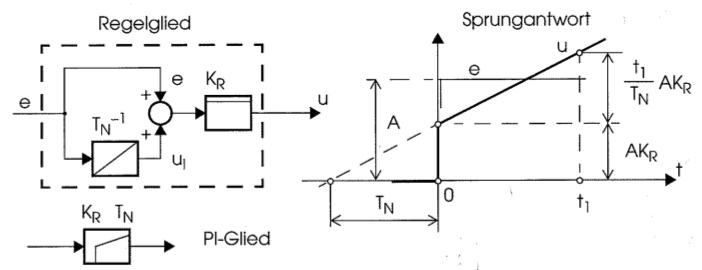
\includegraphics[width=10cm]{./images/PI_Regler.jpg} &
      {\fbox{$G(j\omega)=K_R \dfrac{1+j\omega T_N}{j\omega T_N}$} \newline
       \fbox{$arg(G(j\omega))=\arctan(\omega T_N)-\dfrac{\pi}{2}$}\newline
       \fbox{$|G(j\omega)| = \dfrac{K_R \sqrt{1+(\omega T_n)^2}}{T_n \omega}$}
      \vfill
      }
    \end{tabular}


	\subsection{D-Glied \formelbuch{179/183}}
		Der Differenzierer erzeugt ein Korrektursignal im voraus.
		Nachteilig ist, wenn die Regelgrösse verrauscht ist, dann werden die
		hochfrequenten Störsignale durch die Ableitung verstärkt.\\
		Ein LTI-System, welches ohne D-Glied darstellbar ist, gegebenenfalls durch
		Umformung des Blockdiagramms, heisst realisierbar.  In der Realität wird
		meistens kein reines D-Glied sondern ein $DT_1$-Glied verwendet:\\
		\fbox{$G_{DT_1}(s) = \frac{s T_V}{1+ s T_C}$} \\
    \begin{tabular}{|l||lll|}
      \hline
        \parbox[c][2cm]{3cm}{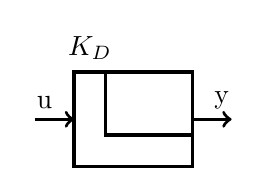
\begin{tikzpicture}
  \begin{scope}[very thick]
    \draw[->] (0,0) -- +(0.5,0) node[near start, above] {u};
    \draw (0.5,-0.6) rectangle +(1.5,1.2);
    \draw[->] (2,0) -- +(0.5,0) node[near end, above] {y};
    \draw(0.9, -0.2) rectangle +(1.1,0.8);
  \end{scope}

  \node at (0.7,0.9) {$K_D$};

\end{tikzpicture}} &
        \parbox[c][2cm]{4.5cm}{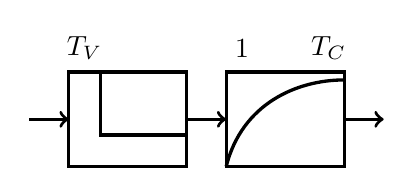
\begin{tikzpicture}
  %D-Glied
  \begin{scope}[very thick]
    \draw[->] (0,0) -- +(0.5,0) node[near start, above] {};
    \draw (0.5,-0.6) rectangle +(1.5,1.2);
    \draw[->] (2,0) -- +(0.5,0) node[near end, above] {};
    \draw(0.9, -0.2) rectangle +(1.1,0.8);
  \end{scope}

  \node at (0.7,0.9) {$T_V$};

  %PT1-Glied
  \begin{scope}[very thick]
    \draw (2.5,-0.6) rectangle +(1.5,1.2);
    \draw[->] (4,0) -- +(0.5,0) node[near end, above]{};
  \end{scope}

   % Zugem�se
   \node at (2.7,0.9) {1};
   \node at (3.8,0.9) {$T_C$};
   \draw[very thick] (2.5,-0.6)  .. controls (2.7,0.2) and (3.4,0.5) .. (4,0.5);

\end{tikzpicture}} &
        $\Rightarrow$ &
        \parbox[c][2cm]{3cm}{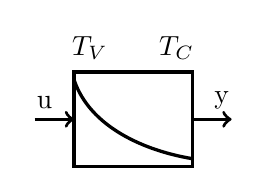
\begin{tikzpicture}
  \begin{scope}[very thick]
    \draw[->] (0,0) -- +(0.5,0) node[near start, above] {u};
    \draw (0.5,-0.6) rectangle +(1.5,1.2);
    \draw[->] (2,0) -- +(0.5,0) node[near end, above] {y};
  \end{scope}

 % Zugem�se
 \node at (0.7,0.9) {$T_V$};
 \node at (1.8,0.9) {$T_C$};
 \draw[very thick] (0.5,0.5)  .. controls (0.7,-0.1) and (1.4,-0.4) .. (2,-0.5);

\end{tikzpicture}}\\
        $D$-Glied &
        $D$-Glied \qquad $PT_1$-Glied & &
        $DT_1$-Glied \\
      \hline
    \end{tabular}
    
    

	\subsection{PD-Regler \formelbuch{187/383}}
    \begin{tabular}{m{10cm}m{8cm}}
      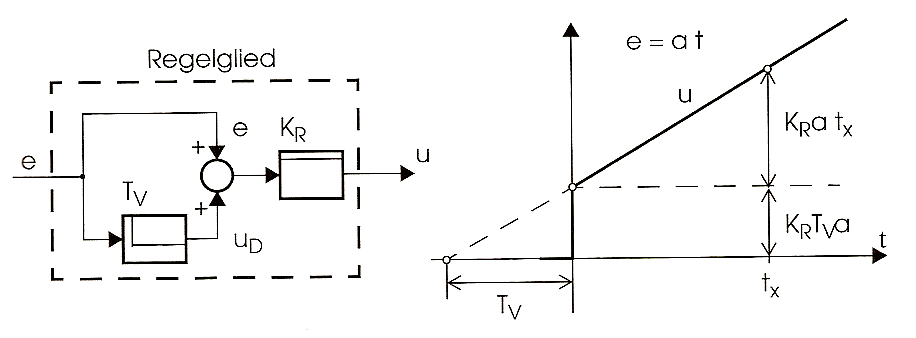
\includegraphics[width=10cm]{./images/PD_Regler.png} &
      {
        Der PD-Regler entspricht dem inversen PT$_1$-Glied. Meistens wird jedoch
        der $PDT_1$ Regler verwendet.\newline
        \fbox{$u=K_R at+K_R T_V a$} \newline
        \fbox{$y = K_R \left(1+\dfrac{T_V}{T_C}\cdot \e^{-\dfrac{t}{T_C}}\right)$} \newline
        \fbox{$G_{PDT_1}(s) = K_R \dfrac{1+s(T_V+T_C)}{1+sT_C}$}
      }
    \end{tabular}
 

	\subsection{PID-Regler \formelbuch{183/383}}
    \begin{tabular}{m{10cm}m{8cm}}
      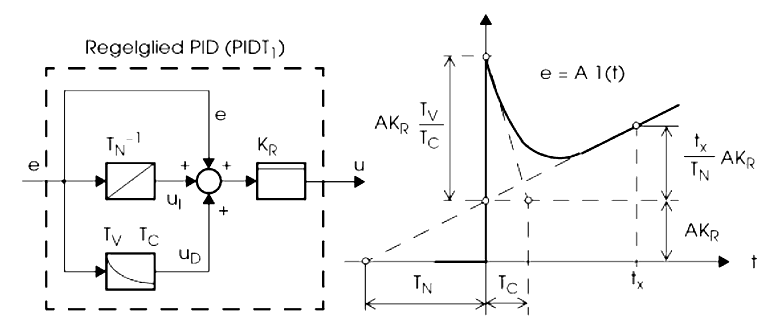
\includegraphics[width=10cm]{./images/PID_Regler.png} &
      {
        \fbox{$G_{PID}(s) = K_R \left(1 + \frac{1}{s T_N} + s T_V \right)$}
        \fbox{$G_{PIDT_1}(s) = K_R \left(1 + \frac{1}{s T_N} + \frac{s T_V}{1+s T_C} \right)$}
      }
    \end{tabular}
		

	\subsection{Empirische Einstellregeln \formelbuch{188}}
		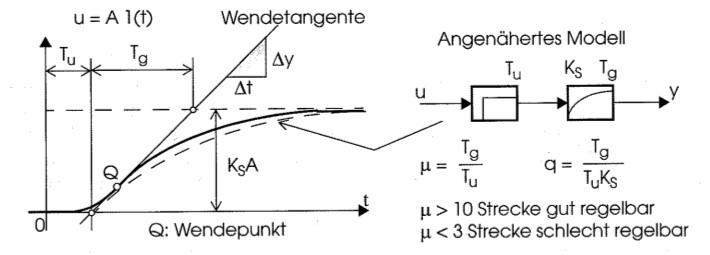
\includegraphics[width=13cm]{./images/Empirisch_Regeln.jpg}
		\begin{minipage}[b]{5cm}
        UTF des angenäherten Modells:\\ \\
		$G_0(j\omega)=\frac{K_s}{1+j\omega T_g}e^{-j\omega T_u}$
		\vspace{2.7cm}
		\end{minipage}\\

	\begin{tabular}{|l|p{1.8cm}|l|l|l|l||l|l|}
	    \hline
	    \multicolumn{6}{|c||}{
	      \textbf{Reglereinstellung nach Chien-Hrones-Reswick}
	    } &
	    \multicolumn{2}{|c|}{
	      \textbf{Reglereinstellung nach Ziegler-Nichols}
	    }
		\\ \hline
		\multicolumn{6}{|c||}{
		  $
		  q = \frac{T_g}{T_uK_S} \qquad \mu = \frac{T_g}{T_u}
		  \qquad \text{wenn} \quad \mu
		  \begin{cases}
		    > 10 \rightarrow \text{Strecke gut regelbar} \\
		    < 3 \rightarrow \text{Strecke schlecht regelbar}
		  \end{cases}
		  $
		} & $q=\frac{T_g}{T_uK_s}$ & $K_{R\pi} \qquad T_\pi=\frac{2\pi}{\omega_\pi}$
		\\ \hline
		\textbf{Regler} & \textbf{Regler\-parameter} &
		\multicolumn{2}{|p{3.5cm}|}{\textbf{Führungsverhalten} \newline $y_m$:
		Überschwingen} &
		\multicolumn{2}{|c||}{\textbf{Störverhalten}} &
		\textbf{Sprungantwort} & \textbf{Stabilitätsgrenze}
		\\ \hline
		& & kein $y_m$ & $\frac{y_m}{y_\infty} = 20 \%$ & kein $a$ & $\frac{a}{b}= 20 \%$ & &
		\\ \hline
		P 	& $K_R$ 	& $0.3q$ 	& $0.7q$ 	& $0.3q$ 	& $0.7q$	& $q$ 	& $0.5K_{R\pi}$
		\\ \hline
		PI	& $K_R$		& $0.35q$	& $0.6q$	& $0.6q$	& $0.7q$	& $0.9q$ 	& $0.45K_{R\pi}$
		\\
		    & $T_N$		& $1.17T_g$	& $1T_g$	& $4T_u$	& $2.33T_u$ & $3.33T_u$ &
		    $0.85T_{\pi}$ \\ \hline
		PID & $K_R$		& $0.6q$	& $0.95q$	& $0.95q$	& $1.2q$ 	& $1.2q$ 	& $0.60K_{R\pi}$
		\\
			& $T_N$		& $1T_g$	& $1.36T_g$	& $2.38T_u$	& $2T_u$ 	& $2T_u$	& $0.50T_\pi$
		\\
			& $T_V$		& $0.5T_u$	& $0.47T_u$	& $0.42T_u$	& $0.42T_u$ & $0.5T_u$ 	& $0.125T_\pi$
		\\ \hline
	\end{tabular}
  
  Empirisch Einstellregeln ergeben praktisch nicht immer das bestmögliche Zeitverhalten,
  sondern sie liefern eine erste Einstellung, welche experimentell noch verbessert werden kann.


	\subsection{Wind-Up \formelbuch{200}}
  \begin{tabular}{lp{15cm}}
    \textbf{Definition:} &
    Der Fehler $e$ am Integratoreingang bleibt konstant, sodass dessen
    Ausgangssignal ständig zunimmt. \\
    
    \textbf{Folge:} & 
    Einerseits ein konstanter Fehler und andererseits eine verzögert reagierende
    und damit stark überschwingende Regelgrösse $y$.
  \end{tabular}

  \begin{multicols}{2}
    \textbf{Ursachen für Wind-Up:}
    \begin{itemize}[leftmargin=*]
      \item I-Anteil
      \item Sättigung am Regler Ausgang
      \item $e(t)$ über "`längere Zeit"' $\neq 0$ ist.
    \end{itemize}
  
  \columnbreak
    
    \textbf{Anti-Wind-Up:}
    \begin{itemize}[leftmargin=*]
      \item Integration beschränken
    \end{itemize}
  
  
  \end{multicols}
  
  

